\section*{Part I -- Why a Continuum Ontology}
\addcontentsline{toc}{section}{Part I -- Why a Continuum Ontology}

\section{Introduction: The Continuum Problem}
\label{sec:r012-continuum-problem}

The Ontology of Continua begins from an ordinary but stubborn fact: real systems
do not respect the disciplinary borders by which they are usually studied. A
factory depends on physics, software, human attention, incentives, supply
chains, security boundaries, and regulation. A living organism depends on
chemistry, cellular architecture, metabolism, signalling, cognition, and
environmental coupling. An AI platform depends on mathematical models, compute
infrastructure, organizational purpose, evaluation regimes, trust, and failure
response. In each case, the object that matters is not merely a thing, a process,
or a dataset. It is a structured continuum that persists while internal
differences, flows, thresholds, and boundaries change.

OC proposes to describe such systems with a shared structural grammar. The
proposal is not that every domain becomes the same, nor that specialist theories
are replaced by a single master vocabulary. The proposal is more modest and more
useful: when different domains speak about persistence, admissible states,
failure, recovery, boundary crossing, feedback, and cross-level dependence, they
often need a common bridge language. Without such a bridge, a physical model, a
biological model, an enterprise model, and a social model may all describe parts
of one system while remaining unable to say how those parts constrain one
another.

\begin{figure}[!htbp]
\centering
\resizebox{0.96\textwidth}{!}{%
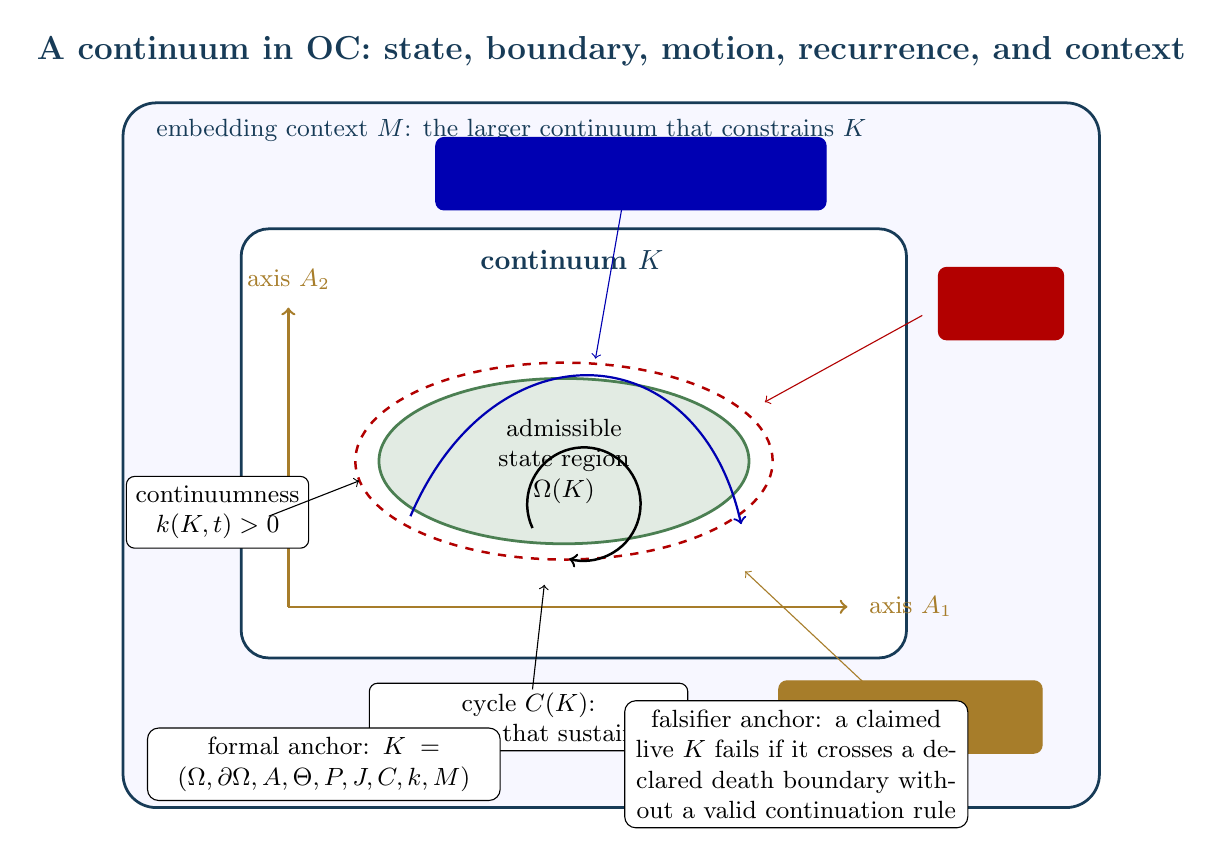
\begin{tikzpicture}[x=1cm,y=1cm, every node/.style={font=\small}]
  \definecolor{ocBlue}{HTML}{173B57}
  \definecolor{ocGold}{HTML}{A77D2A}
  \definecolor{ocGreen}{HTML}{4B7F52}
  \node[font=\bfseries\large, ocBlue] at (0,6.0) {A continuum in OC: state, boundary, motion, recurrence, and context};
  \draw[rounded corners=12pt, fill=blue!3, draw=ocBlue, line width=1.0pt] (-6.2,-3.6) rectangle (6.2,5.35);
  \node[anchor=west, ocBlue] at (-5.9,5.0) {embedding context \(M\): the larger continuum that constrains \(K\)};
  \draw[rounded corners=10pt, fill=white, draw=ocBlue, line width=1.0pt] (-4.7,-1.7) rectangle (3.75,3.75);
  \node[font=\bfseries, ocBlue] at (-0.5,3.35) {continuum \(K\)};
  \draw[->, line width=0.9pt, ocGold] (-4.1,-1.05) -- (3.0,-1.05);
  \node[anchor=west, ocGold] at (3.15,-1.05) {axis \(A_1\)};
  \draw[->, line width=0.9pt, ocGold] (-4.1,-1.05) -- (-4.1,2.75);
  \node[anchor=south, ocGold] at (-4.1,2.86) {axis \(A_2\)};
  \draw[fill=ocGreen!16, draw=ocGreen, line width=1.0pt] (-0.6,0.8) ellipse (2.35 and 1.05);
  \node[align=center] at (-0.6,0.8) {admissible\\state region\\\(\Omega(K)\)};
  \draw[dashed, red!70!black, line width=0.9pt] (-0.6,0.8) ellipse (2.65 and 1.25);
  \node[draw, rounded corners=3pt, fill=white, align=center, red!70!black] at (4.95,2.8) {boundary\\\(\partial\Omega(K)\)};
  \draw[->, red!70!black] (3.95,2.65) -- (1.95,1.55);
  \draw[->, thick, blue!70!black] (-2.55,0.1) .. controls (-1.5,2.55) and (1.1,2.45) .. (1.65,0.0);
  \node[draw, rounded corners=3pt, fill=white, align=center, blue!70!black] at (0.25,4.45) {flow \(J(t)\):\\motion through admissible states};
  \draw[->, blue!70!black] (0.15,4.1) -- (-0.2,2.1);
  \draw[->, line width=0.9pt] (-1.0,-0.05) arc (205:-105:0.72);
  \node[draw, rounded corners=3pt, fill=white, align=center] at (-1.05,-2.45) {cycle \(C(K)\):\\recurrence that sustains \(K\)};
  \draw[->] (-1.0,-2.1) -- (-0.85,-0.77);
  \node[draw, rounded corners=3pt, fill=white, align=center, ocGold] at (3.8,-2.45) {threshold \(\Theta(K)\):\\regime-change surface};
  \draw[->, ocGold] (3.3,-2.1) -- (1.7,-0.6);
  \node[draw, rounded corners=3pt, fill=white, align=center] at (-5.0,0.15) {continuumness\\\(k(K,t)>0\)};
  \draw[->] (-4.35,0.1) -- (-3.2,0.55);
  \node[draw, rounded corners=4pt, fill=white, align=center, text width=0.35\textwidth] at (-3.65,-3.05)
    {formal anchor: \(K=(\Omega,\partial\Omega,A,\Theta,P,J,C,k,M)\)};
  \node[draw, rounded corners=4pt, fill=white, align=center, text width=0.34\textwidth] at (2.35,-3.05)
    {falsifier anchor: a claimed live \(K\) fails if it crosses a declared death boundary without a valid continuation rule};
\end{tikzpicture}}
\caption{A didactic continuum diagram for the external reader. The labels are outside the semantic objects they explain: state region, boundary, axes, flow, threshold, cycle, continuumness, context, formal tuple, and falsifier are all visible without overlap.}
\label{fig:r012-continuum-demonstrator}
\end{figure}

\section{Motivation: Why a Shared Systems Language Is Needed}
\label{sec:r012-motivation}

The wish to describe organized wholes is old. Ancient natural philosophy asked
how form, matter, motion, cause, and purpose relate. Early modern science gained
immense power by isolating mechanisms and measuring them with increasing
precision. Later systems theory, cybernetics, dynamical systems, autopoiesis,
complexity science, network science, formal methods, and enterprise architecture
each recovered part of the same pressure: many important objects are not
adequately understood as isolated components. They are maintained by relations,
feedback, constraints, thresholds, and levels of organization.

The success of specialization created a new difficulty. Scientific fields
became more exact partly by becoming more local. Physics developed languages for
fields, particles, phase transitions, and symmetry. Chemistry developed
languages for reaction networks, catalysis, concentration, and closure. Biology
developed languages for membranes, metabolism, regulation, and evolution.
Cognitive science developed languages for representation, prediction, memory,
and binding. Social theory and economics developed languages for institutions,
markets, incentives, coordination, and trust. Engineering developed languages
for interfaces, requirements, safety, architecture, and operational risk. Each
language is useful. The problem appears when one real system requires all of
them at once.

This is the scientific fragmentation problem in its practical form. The same
world is divided into separate explanatory silos, and each silo often becomes
more precise by reducing how much of the surrounding system it is willing to
represent. OC does not treat that fragmentation as a moral failure of
disciplines. It treats it as a modelling cost that becomes visible whenever
cross-domain prediction, governance, safety, or system design requires several
domains to be held in one account.

The result is a familiar silo pattern. A domain can see its own variables and
miss the constraints imposed by another domain. A technical architecture can be
correct in software terms and fragile in institutional terms. A policy can be
coherent in legal terms and destructive in operational terms. A biological
description can be precise at one level and silent about the higher-level
feedback that changes selection pressure. A strategy can be persuasive in
economic terms and blind to security, cognition, or infrastructure. These are
not merely communication problems; they are modelling problems. If the language
of the model cannot represent cross-domain constraint, the model silently
removes part of the system.

This matters especially as agentic AI systems become more capable. Work that
was once handled by human judgment, tacit context, and informal philosophical
language is increasingly delegated to software agents, model pipelines, and
automated decision loops. Those systems need explicit representations of
state, boundary, evidence, authority, failure, recovery, and cross-level
constraint. If the underlying ontology is shallow, the agent may optimize inside
one domain while damaging another. If the ontology is over-specific, it cannot
generalize. OC is motivated by the need for a middle route: a compact structural
language that is formal enough to be checked and broad enough to describe
systems whose relevant properties span domains.

The economic version of the same problem is equally practical. Enterprises,
governments, laboratories, and platforms all need shared language for complex
systems. A CEO, CIO, enterprise architect, security lead, researcher, and
engineer may discuss the same transformation while meaning different things by
stability, boundary, lifecycle, risk, resilience, and evidence. A useful
meta-ontology should not erase these roles. It should let them translate their
concerns into a common structure: What is the admissible state space? Which
flows sustain it? Which thresholds threaten it? Which cycles maintain it? Which
lower-level continua compose it? Which higher-level continuum contains it?
Which failure would prove the current claim wrong?

The benefit sought by OC is therefore compression without loss of meaning. A
good compression does not flatten a system into a slogan. It preserves the
differences that matter while removing accidental incompatibility between
vocabularies. If a continuum can be described by state space, axes, thresholds,
flows, cycles, boundaries, continuumness, and embedding context, then readers
from different disciplines can at least begin with the same structural map.
They can still disagree about parameters, evidence, interpretation, and
prediction; but they are no longer forced to disagree because their languages
cannot align.

This is also why the manuscript has to be readable before it is merely
checkable. A skeptical reader is right to distrust a theory with a large name if
the opening pages do not explain the problem, the value, and the boundary of
the claim. OC therefore has to earn the reader's patience. It must show why the
same pattern of admissible states, thresholds, cycles, flows, and boundaries
appears in different domains; it must show why that pattern is not already
exhausted by one existing field; and it must state what would make the proposal
fail. The motivation of Core~1.3.3 is not grandiosity. It is the practical need
for a disciplined bridge between domain science, system architecture,
formalization, and evidence review.

\section{Scope of OC Core 1.3.3}
\label{sec:r012-scope}

Core~1.3.3 is a model-core release. It does not claim that every domain
projection is complete, every numerical prediction is validated, or every
formal proof is mechanized. It does claim that the reader-facing manuscript now
contains the public grammar needed to inspect the model: continua, state
spaces, boundaries, thresholds, potentials, flows, cycles, continuumness,
operators, K-levels, proof routes, finite witnesses, retrospective bounded replay QA,
prior-art comparison, and falsifier language.

The included material falls into four classes. First, the conceptual and formal
core states the vocabulary and grammar of the theory. Second, the proof and
formalization layer binds selected claims to proof sheets, Lean-oriented formalization inventory evidence,
finite semantic checks, and counterexample boundaries. Third, the evidence and
reproducibility layer records bounded numerical, replay, comparator, and audit
surfaces. Fourth, the practical and domain layer shows how the model may be read
by engineers, architects, AI builders, strategy readers, and reviewers without
overstating the current science.

The excluded material is just as important. Core~1.3.3 does not promote
unrestricted comparative claim over existing science, declared domain closure, or
complete empirical validation. It does not ask a reader to treat internal build
records as scientific prose. It does not require that every future domain
projection already be complete. It treats missing domain evidence as future
work rather than as a hidden success.

The release is therefore evidence-bounded. A claim is promoted only when its
assumptions, formula or reconstruction rule, proof or evidence class,
comparator boundary, and reopening condition are visible. When the evidence is
finite, scoped, replay-based, or illustrative, the manuscript says so. When a
claim needs broader domain evidence-boundary review or stronger mechanization, that need
remains part of the public limitation.

\section{Conceptual Background Without Duplication}
\label{sec:r012-conceptual-background}

The chapters that follow no longer repeat a second motivation chapter. They
move from motivation into conceptual background. A continuum is introduced as a
structural object; the formal sections later make that object exact. The reader
should keep four questions in view. What makes the system admissible? What keeps
it alive or coherent? What boundary would be crossed by failure? What larger
system contains it, and what smaller systems compose it?


% R012_GOVERNED_PUBLICATION_TRANSLATOR: common service review trace is package metadata, not reader prose.
